\documentclass[../PianoDiProgetto_v3.0.0.tex]{subfiles}

\begin{document}

\section{Pianificazione}
In questa sezione verranno elencate le attività che costituiscono i vari periodi di sviluppo del prodotto. Ogni attività sarà accompagnata da diagrammi che mostrano le tempistiche con le quali deve essere svolta.
	
	\subsection{Primo Periodo - Analisi}
Questo periodo inizia con la formazione del gruppo \kpanic\ e si conclude con la \textbf{\revisionedeirequisiti}\ (RR).\\
\\
\textbf{Periodo: dal 2016/11/28 al 2017/01/11}
\\
\\
Le attività sono le seguenti:
\begin{enumerate}
	\item Scelta degli Strumenti: in quest'attività vengono concordati gli strumenti da utilizzare per la comunicazione  fra i membri del gruppo e quelli da utilizzare per la stesura della documentazione;
	\item Stesura delle \normediprogetto: in questo documento verranno specificate tutte le norme concordate fra i membri del gruppo una volta che sono stati scelti gli strumenti nell'attività precedente. Questo documento viene redatto indipendentemente dal tipo di capitolato scelto;
	\item Si procede alla stesura dei seguenti documenti:
		\begin{itemize}
			\item \studiodifattibilita: si procede alla valutazione tecnica di tutti i sei Capitolati Tecnici proposti, analizzando per ognuno i vari pro e contro. Si procede con la redazione della prima versione del documento \textbf{Studio di Fattibilità}. Al termine di quest'attività viene deciso di comune accordo fra i vari membri del gruppo il Capitolato Tecnico da svolgere;
			\item \pianodiprogetto: si procede alla stesura della prima versione del documento \textbf{\pianodiprogetto}\ nel quale vengono specificate le attività che dovranno essere svolte dal team;
			\item \pianodiqualifica: si procede alla stesura della prima versione del documento \textbf{\pianodiqualifica}\ nel quale si elencano gli obiettivi che il team intende raggiungere e le modalità con le quali intende perseguirli;
			\item \glossario: la stesura della prima versione del documento \textbf{\glossario}\ viene eseguita in modo automatico per quanto riguarda la scrittura dei termini, mentre la loro definizione viene redatta manualmente;
			\item \analisideirequisiti: la prima versione del documento \textbf{\analisideirequisiti}\ viene redatta specificando sia i requisiti tecnici carpiti dal Capitolato scelto, sia i requisiti specificati in seguito dal proponente durante gli incontri pianificati o la comunicazione telematica.
		\end{itemize}	 
\end{enumerate}

	\begin{figure}[!h]
		\centering
		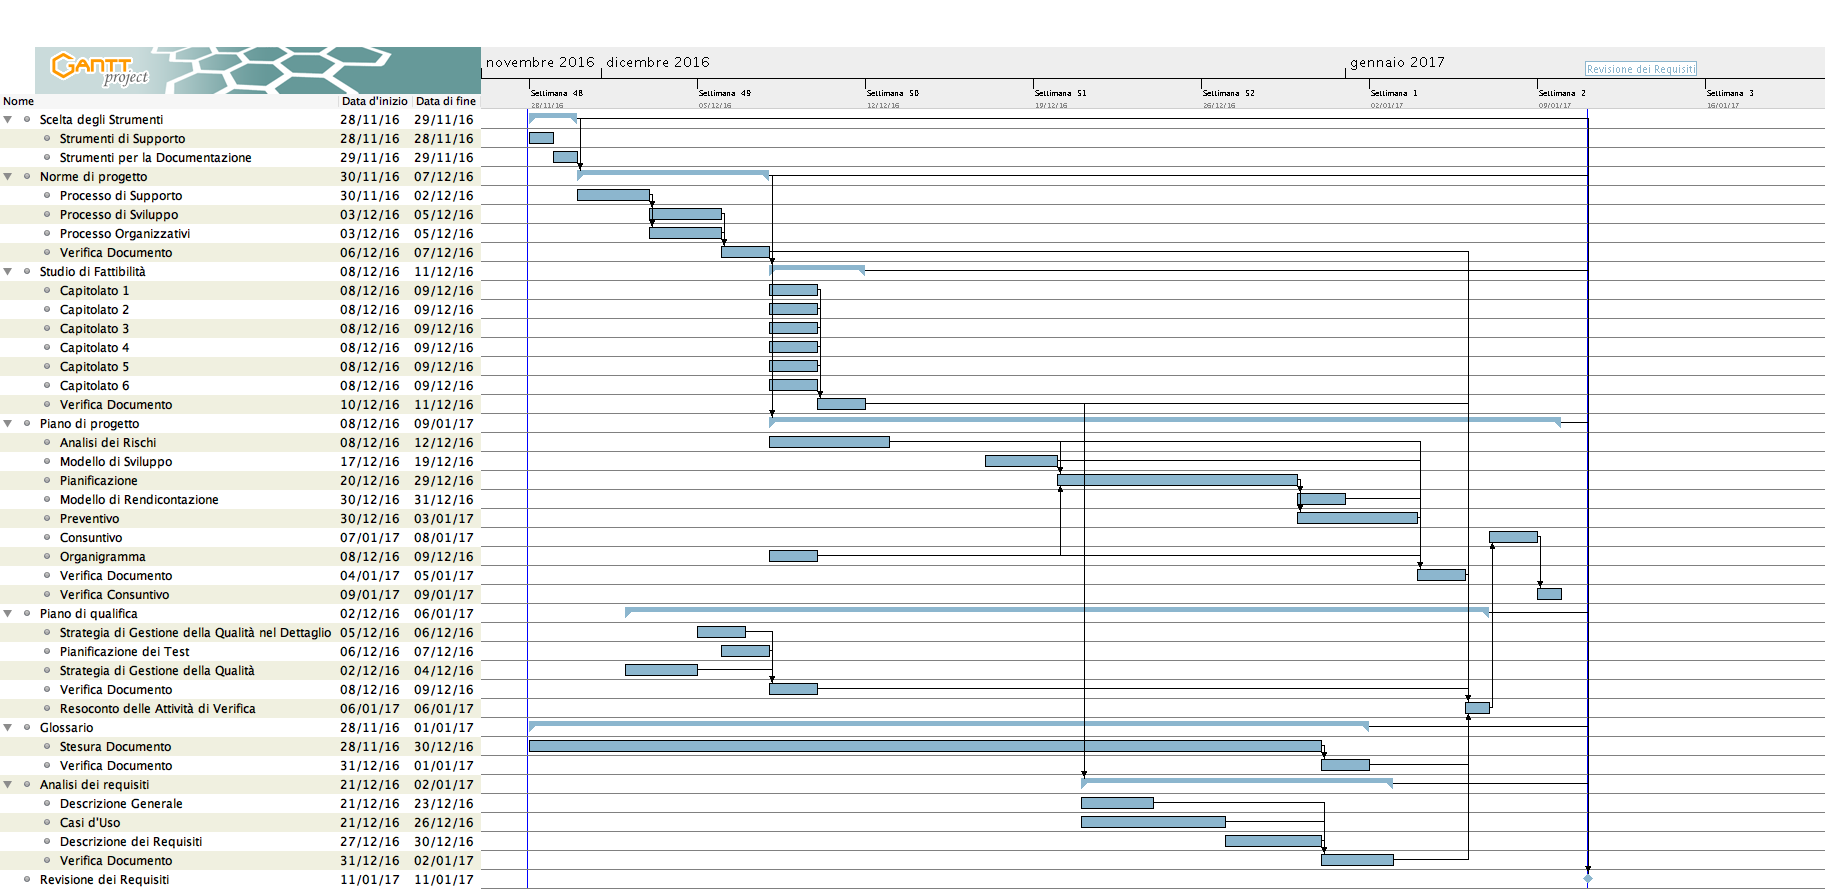
\includegraphics[width=\textwidth]{Pianificazione/Immagini/GanttChart01.png}
		\caption{GanttChart 1}
	\end{figure}	

	\subsection{Secondo Periodo - Analisi di Dettaglio}
	Questo periodo inizia dopo la \revisionedeirequisiti\ e termina con la Milestone prevista per il Secondo Periodo.
	\\
	\\
	\textbf{Periodo: dal 2017/01/25 al 2017/02/03}
	\\
	\\
	Si procede con un incremento della documentazione a seguito della RR. Nei documenti verranno aggiunte anche le specifiche riguardanti eventuali nuove richieste del proponente. Si procede quindi con l'analisi dei requisiti appena individuati.
	
	\begin{figure}[!h]
		\centering
		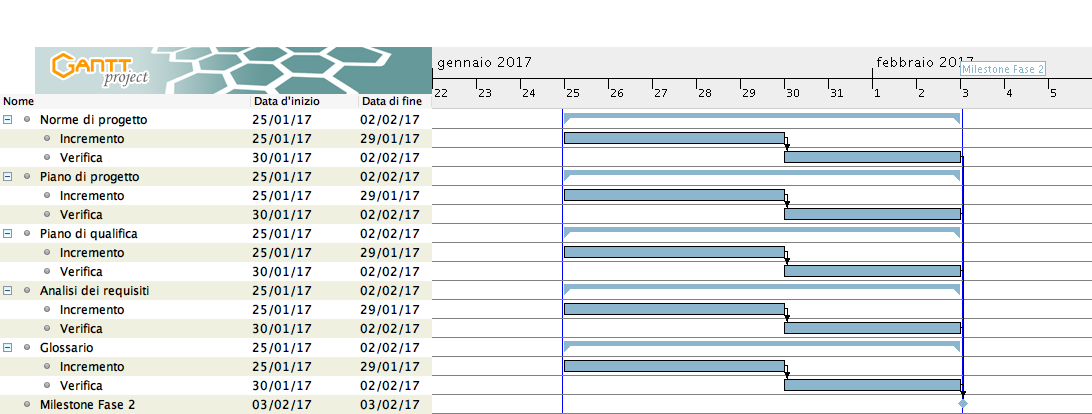
\includegraphics[width=\textwidth]{Pianificazione/Immagini/GanttChart02.png}
		\caption{GanttChart 2}
	\end{figure}	
		
	\subsection{Terzo Periodo - Progettazione Architetturale e Progettazione di Dettaglio}
	Questo periodo inizia dopo la Milestone programmata per il Secondo Periodo e termina con la \revisionediprogettazione\ (RP).
	\\
	\\
	\textbf{Periodo: dal 2017/02/06 al 2017/03/06}
	\\
	\\
	Lo scopo di questo periodo è la stesura della progettazione ad alto livello del sistema e prevede di svolgere le seguenti attività:
	\begin{itemize}
		\item \normediprogetto: il documento verrà modificato e corretto. La versione raggiunta in quel momento sarà la terza;
		\item \analisideirequisiti: il documento verrà modificato e corretto. La versione raggiunta in quel momento sarà la terza;
		\item \definizionediprodotto: la \definizionediprodotto\ viene scritta dal Progettista, il quale descriverà ad alto livello le scelte procedurali prese per il progetto. Saranno quindi descritti quali design pattern verranno implementati, l'architettura logica del software, i principali flussi di controllo, il tracciamento dei requisiti e i componenti hardware per effettuare i successivi test di sistema del prodotto;
		\item \pianodiqualifica: il documento verrà modificato inserendo i dettagli aggiuntivi specificati durante la \revisionedeirequisiti. La versione raggiunta in quel momento sarà la terza;
		\item \pianodiprogetto: il documento verrà modificato apportando correzioni riguardanti la divisione delle attività ed aggiungendo la parte di consuntivo che riguarda quel periodo. La versione raggiunta in quel momento sarà la terza;
		\item Progettazione di Dettaglio: partendo con quando fatto nel Terzo Periodo i \progettisti\ realizzeranno gli schemi in dettaglio che verranno inseriti nella \specificatecnica.
		\item \glossario: il documento verrà modificato inserendo i nuovi vocaboli usati durante l'aggiornamento dei documenti sovra descritti, di cui si ritiene opportuno fornire una definizione. La versione raggiunta in quel momento sarà la terza.
	\end{itemize}
	\newpage
	\begin{figure}[!h]
		\centering
		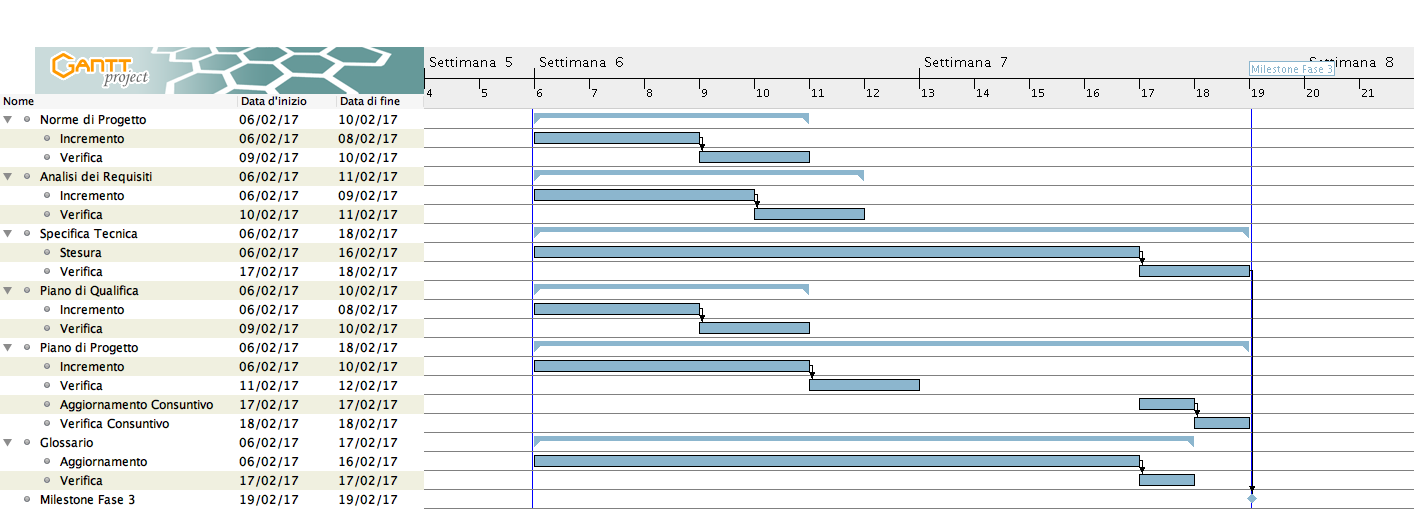
\includegraphics[width=\textwidth]{Pianificazione/Immagini/GanttChart03.png}
		\caption{GanttChart 3}
	\end{figure}	
	
\subsection{Quarto Periodo - Revisione di Progettazione e Codifica dei Requisiti Obbligatori}
	Questo periodo inizia dopo la \revisionediprogettazione\ (RP) e termina con la Milestone prevista per il Quarto Periodo.
	\\
	\\
	\textbf{Periodo: dal 2017/03/14 al 2017/03/31}
	\\
	\\
	L'obiettivo di questo periodo è la stesura, in modo dettagliato, dell'intero sistema, specificando in modo approfondito il comportamento e l'iterazione tra i vari componenti e la realizzazione del codice di cui fanno parte i requisiti obbligatori richiesti dal proponente.
	Si procede con le seguenti attività:
	\begin{itemize}
		\item I seguenti documenti verranno modificati e corretti:
			\begin{enumerate}
				\item \normediprogetto;
				\item \analisideirequisiti;
				\item \pianodiqualifica;
				\item \pianodiprogetto;
				\item \definizionediprodotto
				\item \glossario.
			\end{enumerate}
		La versione raggiunta in quel momento dai documenti elencati precedentemente sarà la terza, mentre la \definizionediprodotto\ raggiungerà la seconda versione;
		\item Codifica dei Requisiti Obbligatori: attenendosi a quanto scritto dai \progettisti\ nel documento \definizionediprodotto, i \programmatori\ dovranno sviluppare il codice del prodotto software che concerne i requisiti obbligatori e desiderabili. L'attività di codifica prevede cicli incrementali per il miglioramento di parti del sistema esistenti o per l'aggiunta di funzionalità al sistema stesso;
		\item Esecuzione dei test: verranno eseguiti sia i test d'integrazione che i test di sistema, secondo quanto previsto dal \pianodiqualifica;
		\item Manuali: si procederà alla stesura del \manualeutente, documento che fornirà un aiuto consistente agli utilizzatori finali del prodotto. Parallelamente verrà redatto anche il \manualesviluppatore.
	\end{itemize}	
		
	\begin{figure}[!h]
		\centering
		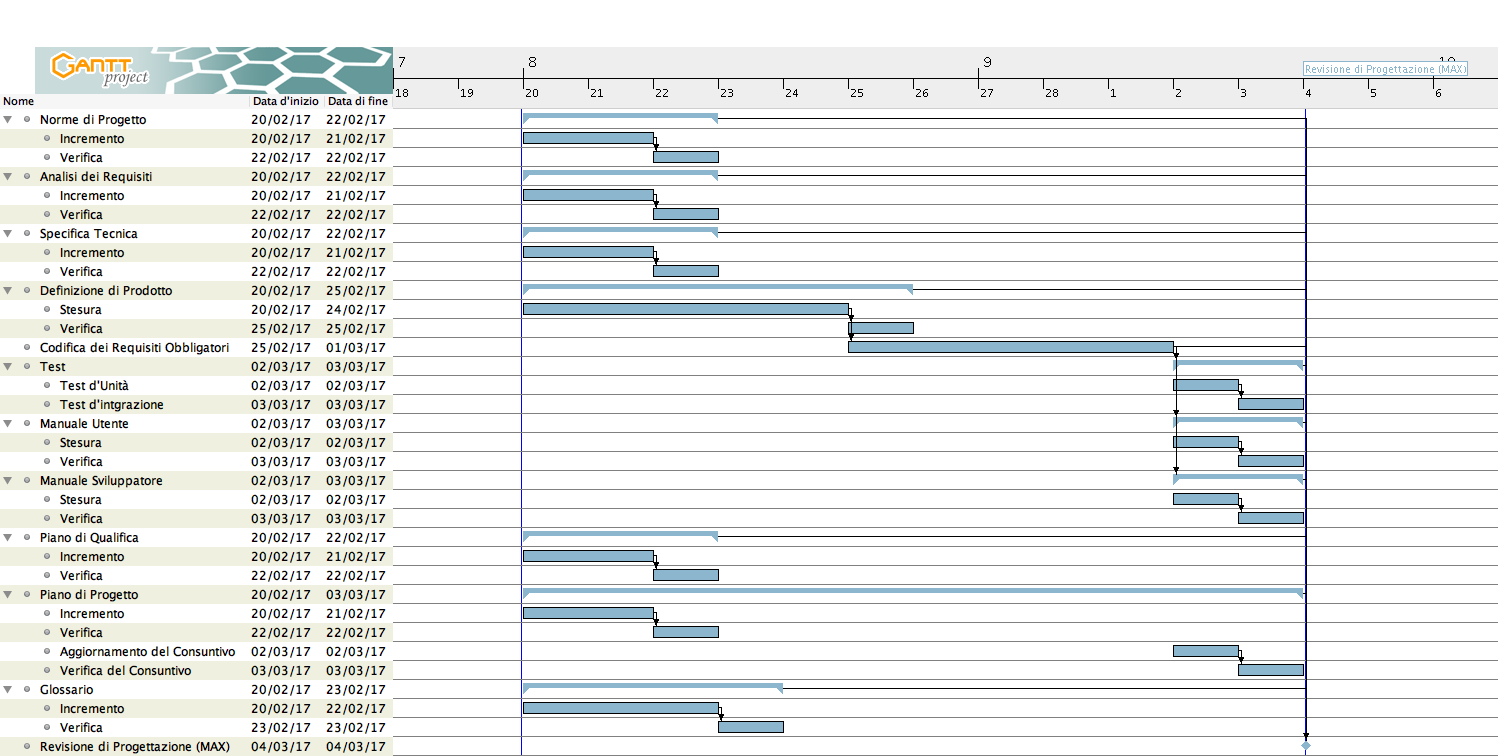
\includegraphics[width=\textwidth]{Pianificazione/Immagini/GanttChart04.png}
		\caption{GanttChart 4}
	\end{figure}	
	
	\newpage
	\subsection{Quinto Periodo - Codifica dei Requisiti Desiderabili}
	Questo periodo inizia dopo la Milestone programmata per il Quarto Periodo e termina con la \revisionediqualifica.
	\\
	\\
	\textbf{Periodo: dal 2017/04/01 al 2017/04/11}
	\\
	\\
	 In questo periodo verrà dedicato alla realizzazione del codice di cui fanno parte i requisiti obbligatori richiesti dal proponente.
	Si procede con le seguenti attività:
	\begin{itemize}
		\item I seguenti documenti verranno modificati e corretti:
			\begin{enumerate}
				\item \manualesviluppatore;
				\item \manualeutente;
				\item \pianodiqualifica;
				\item \pianodiprogetto;
				\item \glossario.
			\end{enumerate}
		\item Codifica dei Requisiti Desiderabili: attenendosi a quanto scritto dai \progettisti\ nel documento \definizionediprodotto, i \programmatori\ dovranno sviluppare il codice del prodotto software che concerne i requisiti desiderabili. L'attività di codifica prevede cicli incrementali per il miglioramento di parti del sistema esistenti o per l'aggiunta di funzionalità al sistema stesso;
		\item Esecuzione dei test: verranno eseguiti sia i test d'integrazione che i test di sistema, secondo quanto previsto dal \pianodiqualifica;		
		\item Manuali: si procederà all'aggiornamento del \manualeutente\ e del \manualesviluppatore.
	\end{itemize}
	
	\newpage
	\begin{figure}[!h]
		\centering
		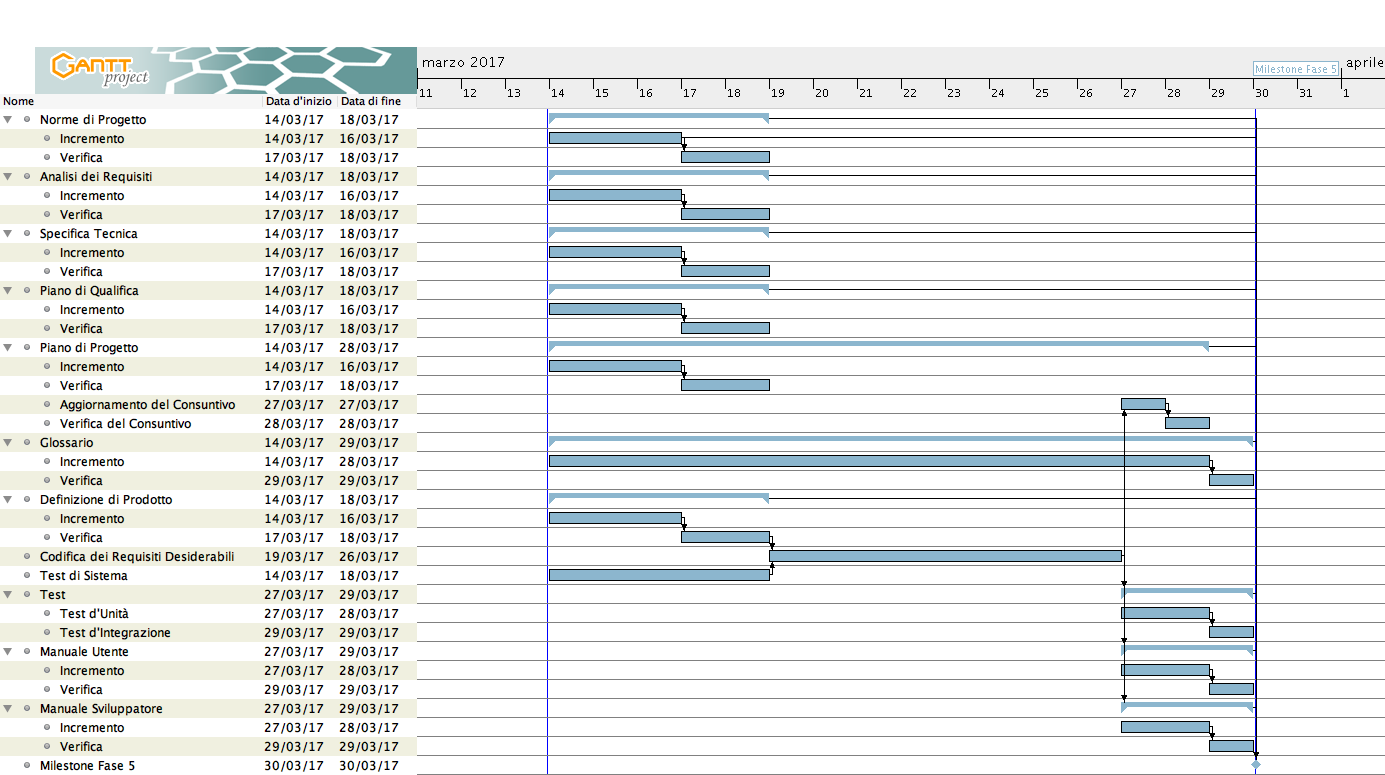
\includegraphics[width=\textwidth]{Pianificazione/Immagini/GanttChart05.png}
		\caption{GanttChart 5}
	\end{figure}	
	
	\subsection{Sesto Periodo - Codifica dei Requisiti Opzionali}
	Questo periodo inizia dopo l'esito della \revisionediqualifica\ e termina con la Milestone prevista per il Sesto Periodo.
	\\
	\\
	\textbf{Periodo: dal 2017/04/19 al 2017/05/02}
	\\
	\\
	Si procede con le seguenti attività:
	\begin{itemize}
		\item I seguenti documenti verranno modificati e corretti:
			\begin{enumerate}
				\item \normediprogetto;
				\item \analisideirequisiti;
				\item \pianodiqualifica;
				\item \pianodiprogetto;
				\item \definizionediprodotto;
				\item \manualeutente;
				\item \manualesviluppatore;
				\item \glossario.
			\end{enumerate}

		La versione raggiunta in quel momento dai documenti elencati precedentemente sarà la quarta, mentre la \definizionediprodotto\ avanzerà alla quarta versione e il \manualeutente e il \manualesviluppatore avanzeranno alle seconda;
		\item Codifica dei Requisiti Opzionali: attenendosi a quanto scritto dai \progettisti\ nel documento \definizionediprodotto, i \programmatori\ dovranno sviluppare il codice del prodotto software che concerne i requisiti opzionali. L'attività di codifica prevede cicli incrementali per il miglioramento di parti del sistema esistenti o per l'aggiunta di funzionalità al sistema stesso;
		\item Esecuzione dei test: verranno eseguiti sia i test d'integrazione che i test di sistema, secondo quanto previsto dal \pianodiqualifica;
		\item Manuali: si procederà all'aggiornamento del Manuale Utente e del Manuale Sviluppatore.
	\end{itemize}
	
	\begin{figure}[!h]
		\centering
		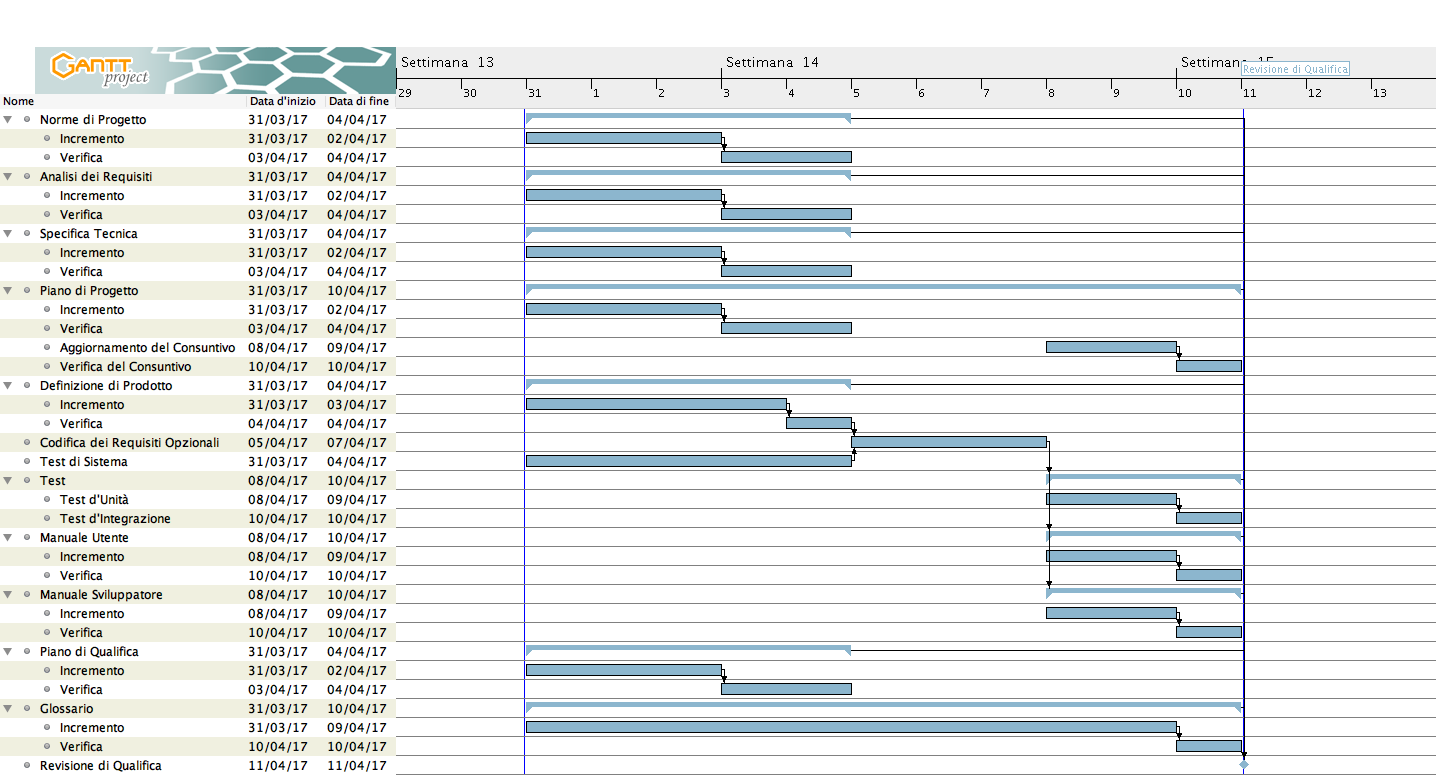
\includegraphics[width=\textwidth]{Pianificazione/Immagini/GanttChart06.png}
		\caption{GanttChart 6}
	\end{figure}	
	
	\subsection{Settimo Periodo - Validazione}
	Questo periodo inizia dopo la Milestone programmata per il Sesto Periodo e termina con la \revisionediaccettazione.
	\\
	\\
	\textbf{Periodo: dal 2017/05/03 al 2017/05/13}
	\\
	\\
	Si procede con le seguenti attività:
	\begin{itemize}
		\item I seguenti documenti verranno modificati e corretti:
			\begin{enumerate}
				\item \normediprogetto;
				\item \analisideirequisiti;
				\item \pianodiqualifica;
				\item \pianodiprogetto.
			\end{enumerate}
		\item Validazione: tramite il tracciamento si verifica di aver soddisfatto i requisiti specificati nell'\analisideirequisiti;
		\item Esecuzione dei test: verranno eseguiti i test finali di sistema, secondo quanto previsto dal \pianodiqualifica;
		\item Collaudo: viene eseguito il collaudo definitivo del sistema creato.
	\end{itemize}
	
	\begin{figure}[!h]
		\centering
		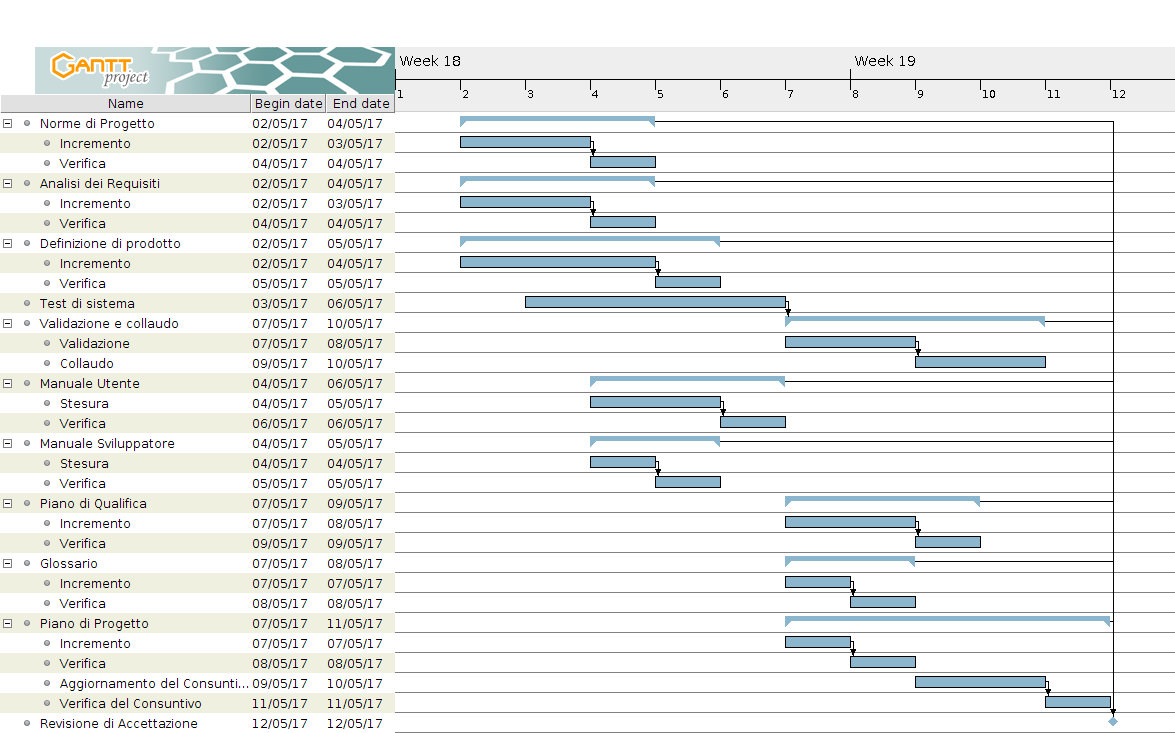
\includegraphics[width=\textwidth]{Pianificazione/Immagini/GanttChart07.png}
		\caption{GanttChart 7}
	\end{figure}	
	
\end{document}